\documentclass[11pt]{amsart}
\usepackage[margin=0.75in]{geometry}                % See geometry.pdf to learn the layout options. There are lots.
\geometry{letterpaper}                   % ... or a4paper or a5paper or ... 
%\geometry{landscape}                % Activate for for rotated page geometry
%\usepackage[parfill]{parskip}    % Activate to begin paragraphs with an empty line rather than an indent
\usepackage{graphicx}
\usepackage{amssymb}
\usepackage{epstopdf}

\DeclareGraphicsRule{.tif}{png}{.png}{`convert #1 `dirname #1`/`basename #1 .tif`.png}

\title{High resolution mapping of magnetic fields in the high-mass star-forming region  G016.96+00.27}

%\date{}                                           % Activate to display a given date or no date

\begin{document}
\maketitle


\section{Scientific Context}
{\bf Context} - It remains still very unclear how dense cores form in filaments and what the role of the  magnetic field is in dense core formation. 
It is statistically identified that Planck Galactic Cold Clumps in filaments exhibit a bimodal distribution of the relative orientation between matter and the magnetic field in the filaments with high density contrast with respect to their environment (Alina et al. 2019).  A detailed polarimetric analysis of individual filaments will bring hints on how the magnetic field influences the formation and evolution of cores in the cold clumps.


{\bf Aims} - We aim to observe the magnetic field at high spatial resolution toward the 
cold core in the massive star forming clump G016.96+00.27 in the Eagle Nebula region:
(1) To follow the magnetic field morphology from Planck observations $\sim$1 pc) down to the core scale (0.1-0.2 pc) probed by SCUBA-POL and HAWC+, 
(2) To evaluate the relative importance of magnetic field, turbulence and gravity by measuring the magnetic field strength, turbulent strength and the mass-to-flux ratio, 
(3) To measure variations in the polarization fraction 
as an indicator of variations in the 3D field structure and the physics of grain alignment (related to field geometry and grain alignment including with regards to column density),  
4) To study the relative magnetic field orientations along filaments to infer the possible 3D field configurations?
and 
(5) To analyze the elongation of cores 
as an indicator of the influence of B-fields on the final mass accretion.

{\bf Methods} - 
We will obtain polarization intensity and orientation from cold dust by using SOFIA's HAWC+ imaging polarimeter in Band E (214 $\mu$m) to be compared with the cloud structure and the 
estimated location of young stellar objects. The plane-of-the-sky magnetic field strength will be obtained using Davis-Chandrasekhar-Fermi method. 

{\bf Synergies} - This work expands on observations made with Planck, the Herschel PACS and SPIRE instruments, and SCUBA-POL by extending polarimetry measurements down to 214 $\mu$m. 
{\bf towards a future ALMA proposal?}

{\bf Anticipated results} - We will produce high spatial resolution maps of the polarized intensity and polarization angles as well as of the 
continuum emission at 214 $\mu$m. 
These maps will be used to constrain models of the 3D cloud and magnetic field structure as well as the grain-alignment physics in conjunction
with Planck, Herschel, and SCUBA-POL data.

\newpage

\section{Scientific Justification}



\subsection{Introduction}

How stars form is one of the most central questions in astrophysics.
It is closely related to major astrophysical problems,
from galaxy structure, formation, and evolution to the dynamics
and chemical evolution of the interstellar medium. It is a complex
process resulting from the interplay between many physical
phenomena including turbulence, magnetic fields, kinematics,
and gravity formation. 
The main parts of the star formation process are understood well, starting from molecular
clouds and progressing via dense cores down to protostellar
collapse (McKee \& Ostriker 2007). This knowledge has
emerged from the detailed observations of the nearest low-mass
and intermediate-mass star formation regions and, in addition,
from sophisticated numerical modelling (Hennebelle et al. 2011;
Padoan \& Nordlund 2011). The next step in improving the overall
view of star formation consists in understanding the process
on the individual scale, and so extensive surveys of stars at different
stages of their formation process and in different environments
are required.

{\bf MJ: The rest of this section one could compress by 50\%, to leave room for description of SCUBA data}

A new approach to the study of the earliest stages of star formation
has been enabled by the Planck satellite (Tauber et al.
2010) that provided
%% This space telescope has mapped the whole sky at several
%% submillimetre wavelengths with high sensitivity and small
%% beam size (below 5 arcmin
%% at the highest frequencies), providing data
%% for 
an all-sky inventory at 5' resolution
of the coldest structures of the interstellar
medium. 

The cold (T$_{dust}$ $\lesssim$ 17 K) and compact (close to beam
size) objects were listed the Planck Catalogue of Galactic Cold Clumps (PGCC, Planck
Collaboration XXVIII 2015), which contains 13188 Galactic
sources. 
This  catalog includes clumps
which possibly host pre-stellar cores and starless cores at subparsec
scales. 
%% Because of the limited resolution, it is dominated
%% by $\sim$1 pc sized clumps and also contains larger cloud structures
%% extending up to tens of pc in size. However, the low temperatures
%% of the objects ensures that only the denser, less evolved
%% regions which are significantly shielded from the interstellar radiation
%% field are included. 
The objects detected by Planck are
likely to contain one or several cores, many of which will be prestellar
or in early stages of protostellar evolution. 

Thanks to its higher spatial resolution, 
Herschel PACS and SPIRE imaging
helped to resolve
%%makes it possible to examine 
the structure of the
sources which gave rise to the Planck detections, often including 
the individual cores. 
%%The inclusion of shorter wavelengths
%%(down to 70 or 100 $\mu$m) helps to determine the physical characteristics
%%of the sources and their environments, and to investigate
%%the properties of the interstellar dust grains. 
%%Galactic
%%cold cores developed by this team (GCC; Juvela et al. 2010), we have mapped selected
%%Planck PGCC objects with the Herschel PACS
%%and SPIRE
%%instruments. 
In this project, we use data obtained from the Hi-GAL Galactic
plane survey (Molinari et al. 2010) and the SPIRE point source catalogue(Schulz et al. 2017) but will carry out more detailed cold core analysis for 
core masses, morphologies, temperature, environments, distances, and evolutionary states following Montillaud et al. 2015.

The addition of core-scale magnetic field studies through polarization
measurements will add to the understanding of how the gravity, magnetic
fields, and turbulence contribute to the formation of pre-stellar cores and how their relative importance may vary from
in different environments.

\subsection{Magnetic field in filamentary dark clouds}

Most massive molecular dark clouds are found to be in filamentary form, with lengths ranging from a couple to more than 10 parsecs. 
Recent state-of-the-art large-scale ideal MHD simulations (e.g., Klassen et al. 2017; Li et al. 2017) of the formation and structure 
of filamentary dark clouds suggest a complicated evolutionary process involving the interaction and fragmentation of 
dense velocity-coherent fibers into chains of cores, resembling observations of nearby clouds (e.g., L1495/B213, Hacar et al. 2013; Musca cloud, Hacar et al 2016; 
Orion ALMA observations, Hacar et al. 2018)

Statistical analysis in the nearby LDN 1642,  Taurus, Musca, Ophiuchus, and Chameleon molecular clouds has revealed 
that the magnetic field tends to be perpendicular to the dense filamentary clouds whereas it tends to be parallel 
at low densities (e.g. Chapman et al. 2011, Cox et al. 2016; Malinen et al. 2016, Planck Collaboration Int. XXXII 2016, Planck Collaboration Int. XXXV 2016). 
This magnetic field alignment is also seen in the recent 850$\mu$m JCMT/POL-2 studies of  G34.42+0.24 (Soam et al. 2019) and 
 and G035.39-00.33 (Liu et al. 2018).
However, most previous near-infrared absorption polarimetry is limited to the low-density, diffuse cloud material with current upper limits, after substantial correction for the known 3-D magnetic field structure, of $A_V \sim 20$ {Kandori et al. 2018). Polarized sub-millimeter thermal dust emission can trace dense region in clouds. 

While Planck sub-millimeter polarimetry is limited due to its low angular resolution (Planck Collaboration et al. 2016), high angular resolution observations of polarized sub-millimeter thermal dust emission on both cloud scales and core scales toward filamentary clouds are still very rare. 
From both optical polarimetry and high angular resolution sub-millimeter polarimetry with CSO and SMA, Li et al. (2015b) found that the magnetic field directions do not change much over the 100 to 0.01 parsec scale in the filamentary cloud NGC 6334, where the fields are not severely affected by stellar feedback. 
They suggest that the self-similar fragmentation in NGC 6334 is regulated by magnetic fields.

Both numerical simulations (e.g., Klassen et al. 2017; Li et al. 2015a) and 
polarization observations (Chapman et al. 2011; Li et al. 2009, 2015b; Zhang et al. 2014; Cox et al. 2016; Pattle et al. 2017 and Ward-Thompson et al. 2017 [BISTRO survey]) 
have suggested that the interstellar magnetic field is dynamically important to the formation of dense cores in filamentary clouds. 

However, it is still very unclear how dense cores form in filaments/fibers and how important the magnetic field is in the formation of dense cores in filamentary clouds compared with turbulence and gravity. Therefore, high resolution sub-millimeter polarimetry observations are urgently needed in order to understand the roles of magnetic field in dense core formation in filamentary clouds and to compare with the state-of-the-art large scale MHD simulations (e.g., Klassen et al. 2017; Li et al. 2017).

{\bf MJ: how the balance between turbulence, gravity, and magnetic fields changes along the cloud evolution and as a function of the scale}

The interstellar radiation field in these filamentary molecular cloud environments is anisotropic due to the shadowing from localized dense ISM regions, thus fulfilling a requirement of  RAT method of grain aligment.

\begin{figure}
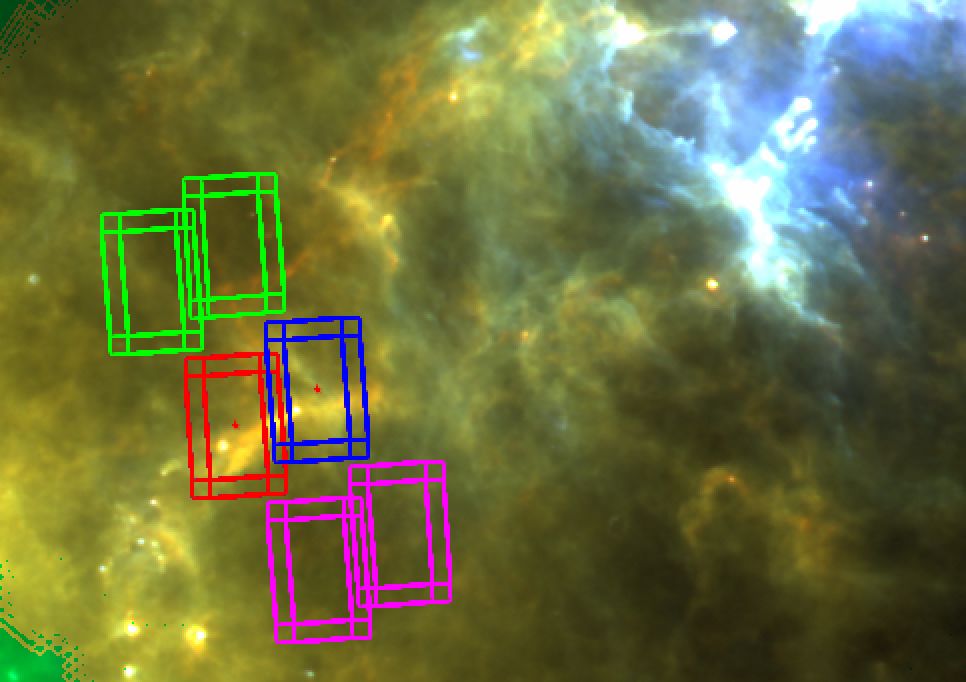
\includegraphics[height=2in]{g16_nmc.png}
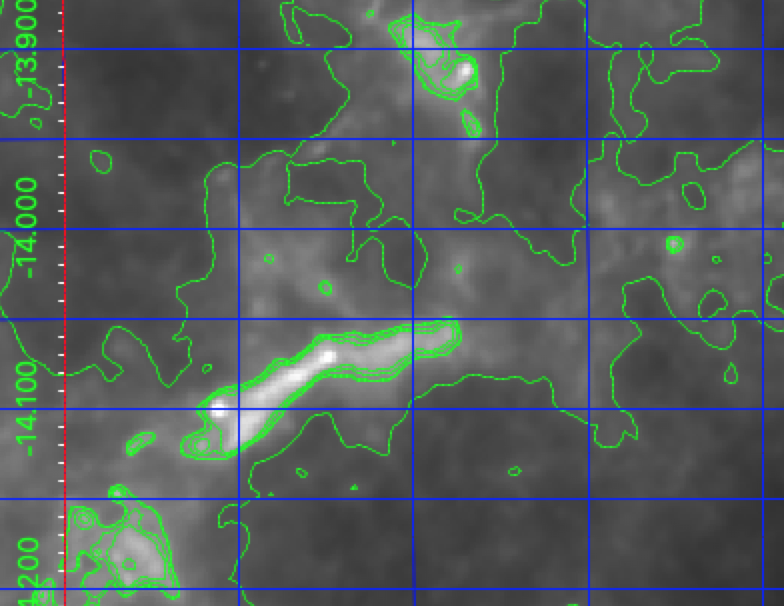
\includegraphics[height=2in]{g16_c3a.png}
\caption{Target field: G16. {\it Left.}  The two NMC mode polarimetry fields are overlaid on an RGB map based on SPIRE 250 micron, PACS 160 micron, and PACS 70 micron imaging.  The hot dust to the East is the famous Eagle Nebula (M16).  {\it Right.} A detail of targeted filament and cores showing contours at SPIRE 250 micron flux densities of 2.6 ($\sigma_{pol} = 3\%$ detection limit), 7.8 ($\sigma_{pol} = 1\%$ detection limit), 8, 9, and 10 Jy/beam. 
\label{fig:fields}}
\end{figure}



\begin{figure}[h]
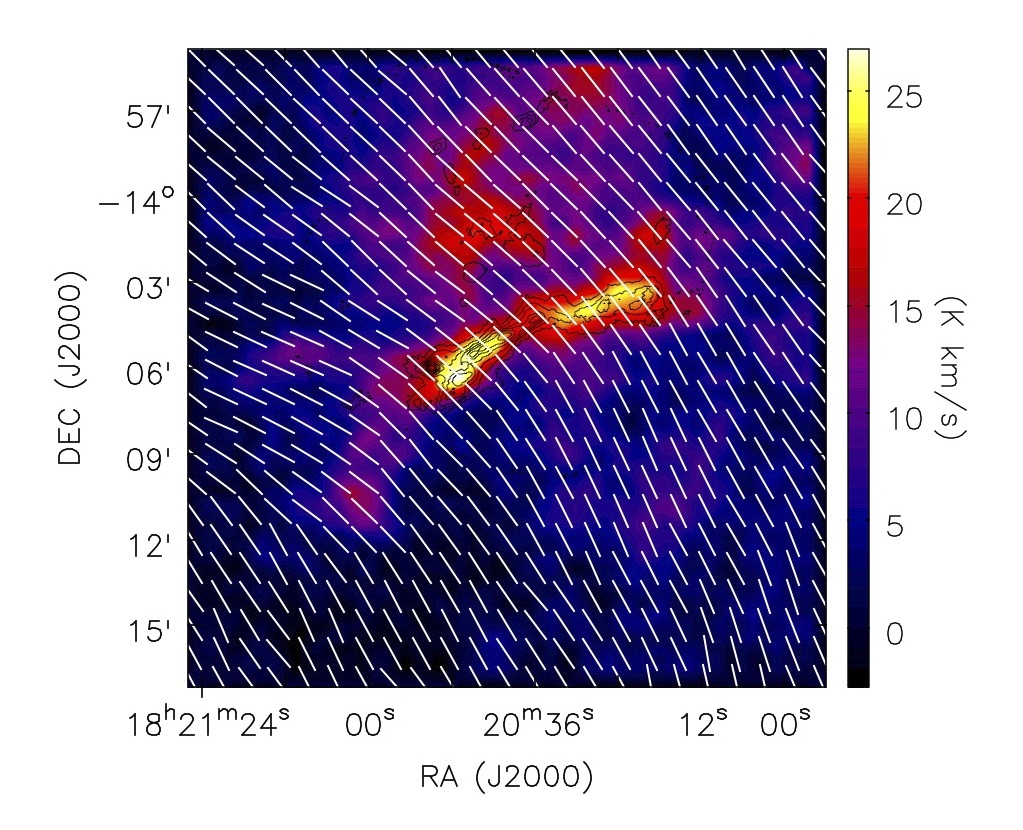
\includegraphics[height=2in]{g16_planckpol.jpg}
\caption{Magnetic field orientation around G016.97+00.27 as inferred from 90 degrees rotation of Planck polarization observations (5 arcmin resolution)
{\bf MJ: there are ~5 vector per beam... a bit too much oversampling?}
{\bf MJ: What is the background image, in line-area units?}
\label{fig:planckpol}}
\end{figure}


\subsection{The importance of SOFIA}

In the post-Herschel era SOFIA offers a nearly unique platform for studies in the Far-Infrared
wavelengths dominated by the spectral features of water present in the terrestrial atmosphere.
At these wavelengths, where the spectral energy distribution of the cold dust associated 
with the earliest stages of star formation peaks, access to altitudes far exceeding those of the
highest earth-bound observatories is required. 

{\bf MJ: from SCUBA-POL and, at large scale, from Planck,}
{\bf MJ: should be differences in the polarisation fraction and polarisation angles between}

The combination of this observatory providing FIR polarization measurements
with submillimeter data, will enable study of the SED of the polarized dust emission and to check for wavelength dependence in the derived polarization angles
There could theoretically be some difference between 214$\mu$m and 450/850 $\mu$m because of the different contributions of carbonaceous and silicate grains  and because 850$\mu$m would be more sensitive to cold dust while 214$\mu$m is weighted more towards the warmer surface layers, giving rise to differences in the measured polarization angles.

 
\subsection{Target selection}

In this proposal we seek to study the role of magnetic fields in the formation of pre-stellar cores within 
nearby giant molecular clouds.
We will evaluate the relative importance of magnetic field, turbulence and gravity by measuring the magnetic field strength, turbulent strength and the mass-to-flux ratio.

From the set of sources for which we have Herschel imaging, and for which we have or will obtain polarization data at  450 and 850 microns from JCMT/POL-2, included as part of JCMT SCOPE survey of 1000 PGCCs (Liu et al. 2018), we consider those that are within 2 kpc, have Declinations north of -15 degrees, and that are not subject to line of sight confusion. The distance limit corresponds to a resolution better than the typical 0.2 parsec core scale given the HAWC+ Band E FWHM of 18.2 arcsec. 

The GMC that we select is G16.96+0.27 (G16) from the JCMT SCOPE survey. It is among brightest 850 $\mu$m sources in the SCOPE catalog and hence appropriate for JCMT/POL-2 observations. G16 is a structurally simple and largely quiescent cloud near the Eagle Nebula (M16) at a distance of 1.8 kpc. 
The BISTRO program has observed the much fainter Pillars of Creation in M16 successfully so POL-2 detections are assured for G16 (Pattle et al. 2018).

$^{13}$CO spectra 
obtained using the JCMT over a 5-arcminute patch
show a single velocity component at  $\sim$25 km s$^{-1}$, indicating that no cloud confusion is present along the line of sight. The western bright core is associated with the massive protostar MSX6C G016.9261+00.2854 (Urquhart et al. 2011).


Additional ancillary data on hand include $^{12}$CO(1-0), $^{13}$CO(1-0), and C$^{18}$O(1-0) line studies at 0.3 km s$^{-1}$ resolution from the TRAO 13.7m, 
and extensive astrochemical studies using the NRO 45m of N$_2$H$^+$, CCS, HC$_3$N, DNC, HN$^3$C, N$_2$D$^+$, and cyclic-C$_3$H$_2$ at 
0.05 km s$^{-1}$ resolution (Tatematsu et al. 2017).

In Figure \ref{fig:fields} we present the field using SPIRE 250 $\mu$m and PACS 70 and 160 $\mu$m imaging. At high column densities, the observed polarization fraction could be low, even down to ~1\%, but high surface brightness still results in SNR$>>$3. At lower surface brightness the polarization fractions are typically higher, because of less magnetic field tangling or stronger grain alignment. At 5 arcmin scale, Planck observes in these regions polarization fractions of some 3\%
with inferred magnetic field directions perpendicular to the filament.

{\bf MJ: need further information on the filament (column density, temperature, length, width), perhaps including a larger figure showing the column densities at \~HAWC+ resolution (and the SCUBA-POL polarisation vectors)
}



\clearpage

{\bf References.} 
\\
\\
Alina, D. et al.  2019,  MNRAS, 485, 2825 \\
Chapman, N. et al. 2011, ApJ, 741, 21 \\
Cox, N. L. J. et al. 2016, A\&A, 590, 110 \\
Hacar, A. et al. 2013, A\&A, 554, 55 \\
Hacar, A. et al. 2016, A\&A, 587, 97 \\
Hennebelle, P. et al. 2011, A\&A, 528, A72 \\
Juvela, M.  et al. 2010, A\&A, 518, L93 \\
Kandori, R. et al. 2018, ApJ, 857, 100 \\
Klassen M. et al. 2017, MNRAS, 465, 2254 \\
Li, H.-B. et al. 2015a, MNRAS, 452, 2500 \\
Li, H.-B. et al. 2015b, Nature, 520, 518L \\
Liu, T. et al. 2018, ApJS, 234, 28 \\
Liu, T. et al., 2018,  ApJ, 859, 151 \\
Luhman, K. L. 2001, ApJ, 560, 287 \\
Malinen, J. et al. 2014, A\&A, 563, 125 \\
Malinen, J. et al. 2016, MNRAS 460, 1934 \\
McGehee, P. M. 2008, in Handbook of Star Forming Regions, Vol. II, ed. B. Reipurth, 813 \\
McKee \& Ostriker 2007, ARA\&A, 45, 565 \\
Molinari, S.  et al. 2010, PASP,  122, 885 \\
Montillaud, J. et al. 2015, A\&A, 585, A92 \\
Pattle, K.  et al. 2017, ApJ, 846, 122 \\
Pattle, K.  et al. 2018, ApJ, 860, L6 \\
Pattle, K. et al. 2019, ApJ, 880, 27 \\
Padoan \& Nordlund 2011, ApJ, 730, 40 \\
Planck Collaboration et al. 2016, A\&A, 586, 138 \\ 
Planck Collaboration Int. XXXII 2016, A\&A, 586, A135 \\
Planck Collaboration Int. XXXV 2016, A\&A, 586, A138 \\
Planck Collaboration XXVIII 2016, A\&A Volume 586 \\
Planck Intermediate Results L.  2017, A\&A 599, A51 \\
Rapson, V et al. 2014 ApJ 794 12 \\
Santos et al., ApJ accepted, arXiv:1905.00705 \
Soam, A. et al. 2019, arXiv:1908.03624\\
Schulz, B. et al. 2017, arXiv:1706.00448 \\
Tatematsu, K. et al. 2017, ApJS, 228, 12\\
Tauber, J.  et al. 2010, A\&A, 520, 1 \\
Urquhart et al. 2011, MNRAS, 485, 1685\\
Ward-Thompson, D. et al. 2017,  ApJ, 842, 66 \\
Zhang, Q., et al. 2014, ApJ, 792, 116

\newpage
\section{Feasibility and the Path to Publication}

\subsection{Mapping and estimated exposure times\label{sec:exptime}}

The Band E HAWC+ beam at 18.2 arcsec FWHM offers identical angular resolution to the Herschel SPIRE observations
and thus we expect that the continuum and polarization maps from SOFIA will also well resolve these dense cores.
The proposed observations will allow us to examine whether magnetic fields are perpendicular to the main filament long axis as predicted in simulations (Li et al. 2017) and also as observed in nearby low-mass clouds (e.g., L1495/B213; Chapman et al. 2011). 
By comparing with the Planck data, we will investigate how magnetic field directions change from the 
cloud scale (1 pc) down to the core scale (0.1-0.2 pc) and hence establish whether the formation and fragmentation of these cold structures are also regulated by magnetic fields.
{\bf MJ: whether this changes towards the central filament (as suggested by numerical simulations) or is affected by the fragmentation and accretion onto cores}

We assume a standard $\beta$=1.8 dust and consider the 160/250 $\mu$m flux density ratio from the PACS and SPIRE maps. 

For 10 points selected along the filament, on the two bright cores, and in the extended northern emission, we find ratios between 0.34 and 0.65, with a mean of 0.42. These correspond to temperatures of 10.0 to 12.6 K, with the mean ratio implying a characteristic temperature of 10.8 K.  
The corresponding 214/250 $\mu$m flux density ratios are then 0.80 to 0.98, with the mean value mapping to a {\bf 214/250 $\mu$m ratio of 0.86} which is used here.
 
The primary observations proposed are HAWC+ NMC mapping in polarimetric mode. 
{\bf Note that we are proposing for chop-nod but we will accept the observation in OTF mode.}
Four hours of continuous observation time, after consideration of overlap in USPOT, result in 5120 seconds (or 16 AOR repeats with a 40 second full nod pattern) of
integration time. With default observing conditions, the SITE tool informs us that the flux density limit for obtaining SNR=3 at $\sigma_{pol}  = 1\%$
is 0.0142 Jy/arcsec$^2$ in Band E. 

Conversion from 214 $\mu$m flux density into that at 250 $\mu$m, and then in SPIRE map units of Jy/beam gives a {\bf detection limit of 7.8 Jy/beam}
given the 470 arcsec$^2$ SPIRE beam size.  In the lower column density regions where polarization fractions of $\sim3\%$ are expected, in the same
observation we can reach down to 2.6 Jy/beam contour, enabling mapping of the extended emission notably to the north of the filament.

In order to map both the east and west sides of the filament, we propose to observe two overlapping FOVs. These are centered 1\' north of the filament to include
the fainter extended emission. Given the complex structure of the region we propose a chop throw of 500\" at an angle of 30$^o$. 
The total required observation time is 8 hours, split between two 4-hour fields.


\subsection{Analysis}
Upon receipt of the calibrated data, there are a number of tasks that the team will undertake in order
to create a comprehensive view of the star formation processes in these different environments. This team has a number of recent publications dealing with analysis of submillimeter and far-IR polarization data from Planck and JCMT/POL-2 - these are listed below.

Issues that we have dealt with include the effect of measurement noise in polarization data with data from the Planck mission covered in a series of papers led by L. Montier and D. Alina.
In these investigations, the parameter bias in the presence of measurement noise is addressed. It is critical to take into account all the information available in the data in order to accurately derive these polarization parameters.  In our previous work, we studied the bias on polarization fraction and angle, various estimators of these quantities, and their associated uncertainties. {\bf MJ: }This experience is used when estimating the reliability and the parameter biases in the HAWC+ data.}

In the context of JCMT/POL observations, we have studied especially the massive IRDCs 035.39-00.33 and 034.43+00.24, where POL-2 data showed clear changes in magnetic field orientation relative to the main filament and its cores  (Liu et al. 2018, Soam et al 2019). 
Detailed 3D radiative transfer modelling was used to examine  how the polarization angles and fractions depend on potential magnetic field geometries and grain alignment (Juvela et al. 2018).
{\bf MJ: Similar analysis will be carried out using the HAWC+ data, supported by the existing SCUBA-POL and Planck measurements.}
In addition, the Herschel sources seen in the G016 field will have their core properties calculated following the methods used in Montillaud et al. 2015 and the combined data will be used for dust evolution studies.
{\bf MJ: to measure variations in dust opacity and the dust opacity spectral index}

We will compare the HAWC+ Band E  polarization maps with those from Planck data
 to understand the magnetic field behavior on spatial scales ranging from the cores out to filaments and the
entire cloud. These polarization results will be interpreted in the context and environment of each 
targeted core and against models of dust evolution. 

The observed polarization fraction might depend on dust properties, mainly grain sizes, and thus would be linked to 
the physical conditions and the evolution history of the objects (Santos et al. 2019, Pattle et al. 2019)

%This is for Carina, a GMC at 3.3 kpc.
% Shariff et al. 2019, ApJ 872 197
%
% an interesting result that the BLAST-Pol team has been seeing is a flat polarization spectrum across the submillimetre, unlike previous work which found a minimum %at 350$\mu$m.  However, their results are entirely for nearby, low-mass clouds (I think).  This study might be the first opportunity to test this in high-mass star-forming %regions.

We will combine this analysis with the structure evidenced with Herschel
at intermediate scale, including striations, filaments and cores at different evolutionary stages.
This is a multi-parameter analysis which will include consideration of core mass, morphology, and temperature;
the surrounding radiation field; and the mass, column density, and morphology of the parent cloud and the intermediate scale features within it.
We will also carry out 3D radiative transfer modeling to study the effect of magnetic field geometries, dust property variations, and the grain alignment efficiency in the field, similarly to Juvela et al. (2018).
 


\end{document}  